\chapter{Compositional Refinement of Inferred Specifications}
\label{ch:article3}

\noindent\textbf{Preface.} The single-pass heuristic inference of the earlier
chapters is necessarily local: it reasons about a method in isolation. This
chapter asks whether a second, \emph{compositional} pass---propagating
weakest-precondition obligations across method boundaries---recovers
specifications a single pass misses, and measures the effect on a large corpus.
It establishes that compositional refinement strictly extends heuristic inference,
yielding a substantial number of additional well-formed preconditions. This result
is pivotal twice over: it strengthens the inference instrument, and it supplies the
mechanism on which behavioural version-compatibility analysis later rests, because
the same compositional reasoning that recovers a caller's obligations from a
callee's contract is what lets a contract change be propagated across a call graph
(Chapter~7). The candidate led all aspects of the study; the advisors contributed
review. The chapter is reproduced below as submitted, in double-blind form, to the
\emph{International Conference on Software Engineering}.
% TODO: replace the anonymised submission PDF with a de-anonymised version for the
% examined thesis, since the thesis is not blind-reviewed.

\cleardoublepage
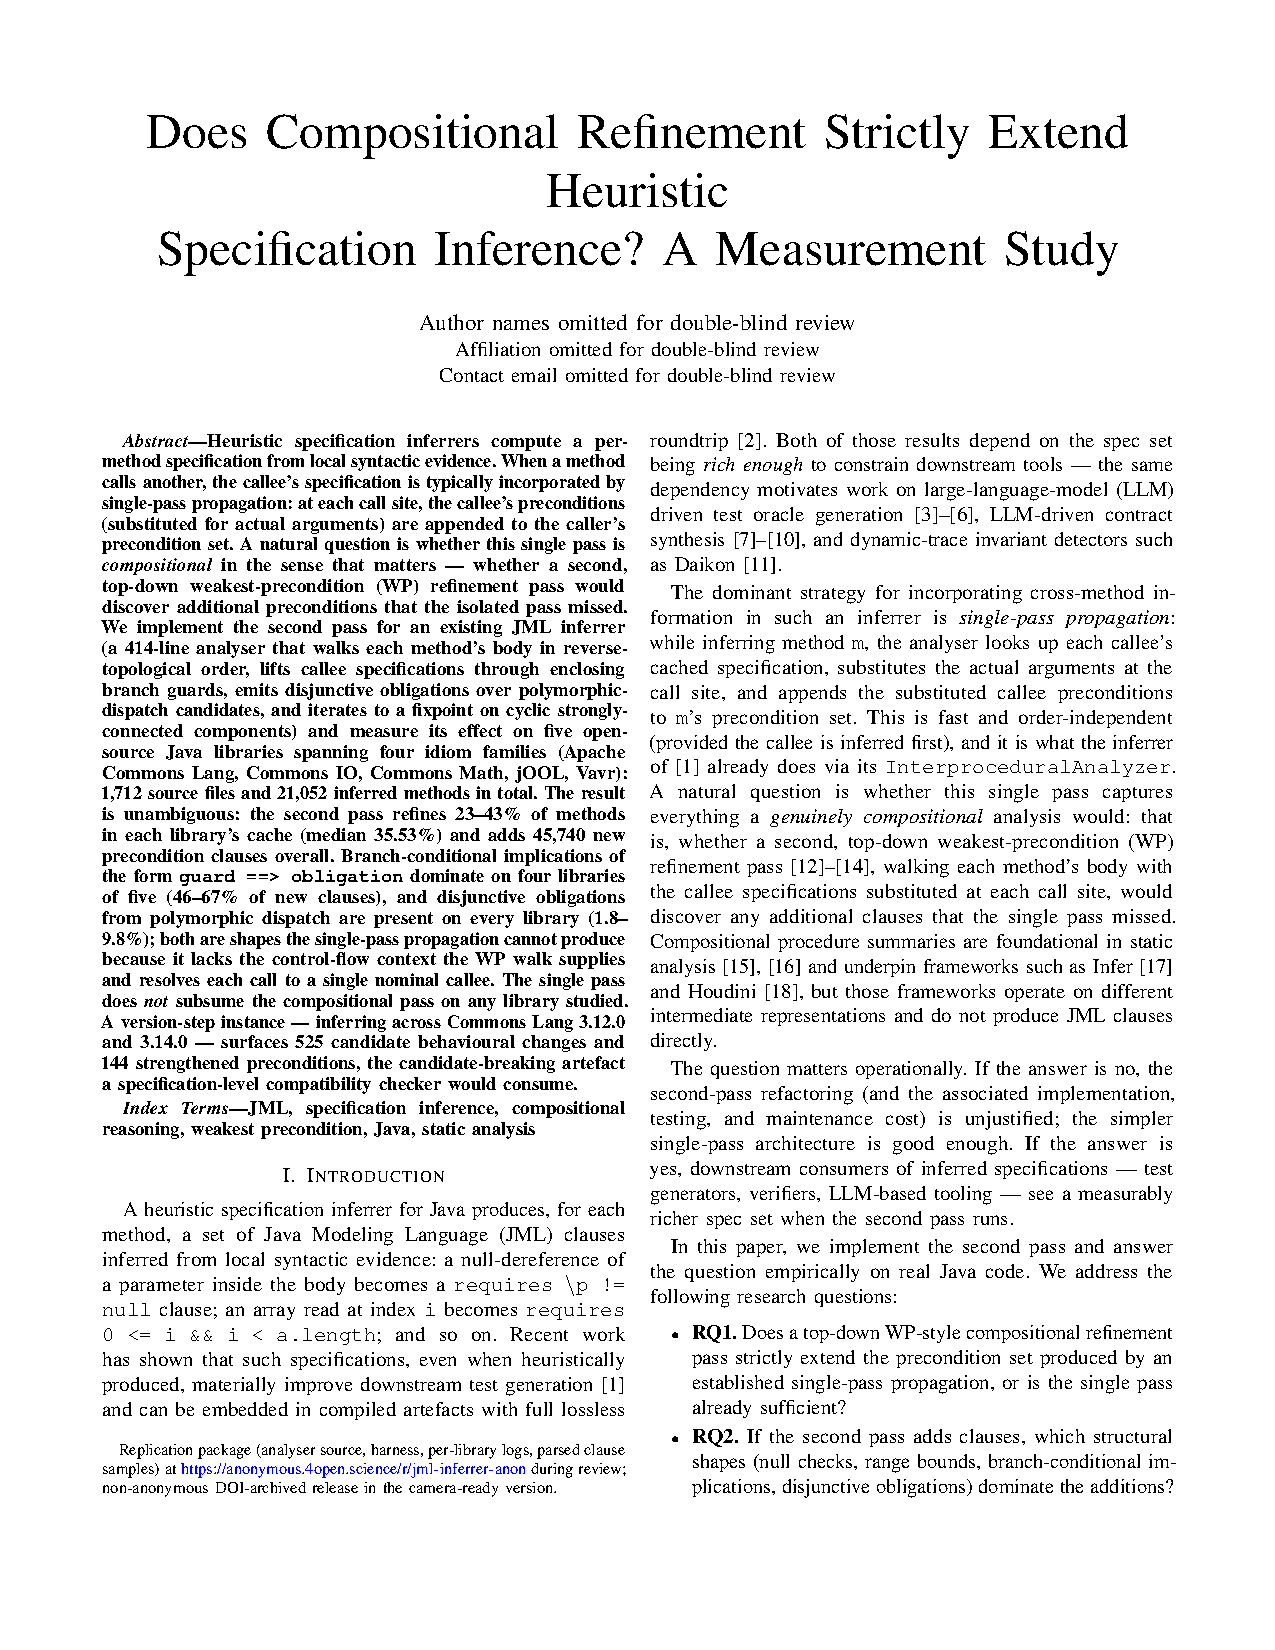
\includepdf[pages=-,width=\textwidth]{../article3/article3.pdf}
